\documentclass[french,12pt]{article}
\usepackage[utf8]{inputenc}
\usepackage{indentfirst}
\usepackage[T1]{fontenc}
\usepackage[a4paper,left=2cm,right=2cm,top=2cm,bottom=2cm]{geometry}
\usepackage[french]{babel}
\usepackage{listings}
\usepackage{hyperref}
\usepackage{libertine}
\usepackage{libertine}
\usepackage{tikz}
\usepackage{float}
\usepackage{amsmath}
\usepackage[linesnumbered,ruled,french,onelanguage]{algorithm2e}
\makeatletter 
\g@addto@macro{\@algocf@init}{\SetKwInput{KwOut}{Sortie}} 
\makeatother
\usepackage[pdftex]{graphicx}
\usepackage[export]{adjustbox}
\usepackage{mathtools}
\usepackage{subfig}

\usepackage{qtree}

\setlength{\parskip}{1ex plus 0.5ex minus 0.2ex}
\newcommand{\hsp}{\hspace{20pt}}
\newcommand{\HRule}{\rule{\linewidth}{0.5mm}}

\begin{document}

\begin{titlepage}
  \begin{sffamily}
  \begin{center}

    % Upper part of the page. The '~' is needed because \\
    % only works if a paragraph has started.
    
\includegraphics[scale=0.94]{unicaen.png}~\\[1.5cm]

    \textsc{\LARGE Université de Caen Normandie}\\[2cm]

    \textsc{\Large Rapport de Projet}\\[1.5cm]

    % Title
    \HRule \\[0.4cm]
    { \huge \bfseries Les tables du spectre visible\\[0.4cm] }

    \HRule \\[2cm]


    % Author and supervisor
    \begin{minipage}{0.4\textwidth}
      \begin{flushleft} \large
        Jules DUBANET,\\ Emilien BLONDEAU,\\ Christopher BAUDOUIN,\\ Bintou DIAKITE\\
        Mars 2023\\
      \end{flushleft}
    \end{minipage}
    \begin{minipage}{0.4\textwidth}
      \begin{flushright} \large
        \emph{Superviseur:} M. BONNET \textsc{Gregory}\\
        
      \end{flushright}
    \end{minipage}

  \end{center}
  \end{sffamily}
\end{titlepage}



    \tableofcontents

\newpage


    \section{Introduction}

    
    Le but de ce projet était d'expérimenter sur une alternative au craquage de mot de passe dit "brute force" avec les Rainbow Tables, ou tables arc-en-ciel en français (on dira RBT dans la suite de ce rapport). Ce sont des structures de données censées représenter un grand nombre de mots de passe ainsi que leurs haché, tout en ayant une complexité en espace plus raisonnable qu'en stockant directement tout ces couples mots de passe/haché en clair.
    Ces tables servent à tenter\footnote{L'attaque avec une RBT peut effectivement échouer, là ou un bruteforce ne subira jamais d'échec.. du moins si on lui laisse une infinité de temps.} de retrouver un mot de passe à partir d'un haché, prélevé au préalable dans une base de données par exemple. 
    \newline
    \indent Dans ce rapport nous allons d'abord vous présenter l'objectif de ce projet (quelle problématique engendrent les RBT), une rapide description des fonctions implémentées ainsi que de l'organisation du projet, une explication plus précise des éléments techniques de ce projet, puis l'architecture de celui-ci. On finira par montrer nos expérimentations et ses résultats, en les analysant, essayant de voir s'ils répondent à notre problématique.


  \section{Objectifs du projet}
        Dans ce projet, l'objectif principal était d'implémenter les RBT afin d'expérimenter sur celles-ci pour pouvoir répondre aux questions sur l'efficacité des RBT: \textit{\textbf{"Quelle est l'efficacité de la table en fonction du nombre de couleurs, de sa taille et de la taille des mots de passe ?"}}. On peut, de plus, se demander si ces trois facteurs se valent, ou si certains sont plus intéressants que d'autres. 
        \newline
        \indent
        Pour implémenter les RBT, il y a plusieurs points clés: il nous faut d'abord des fonctions de réductions et de hachage. Ensuite, nous avons besoin de créer une grande base de mot de passe et de quoi générer les RBT à partir de tout ça. Et enfin nous devons implémenter un algorithme pour réaliser une attaque à partir de celle-ci. Des problèmes sous-jacents émergent tels que : comment représenter nos RBT? Quels formats de fichier utiliser ? Un ou plusieurs fichiers ? Ces problèmes se sont effectivement manifestés tout au long de notre développement.
        \newline
        \indent
        De nombreuses explications et de nombreux travaux existent déjà sur le sujet, lesquels nous ont servis à la base de notre projet pour bien comprendre le concept de RBT\cite{ArticleMieuxCoder}\cite{WikiRBT}. L'article sur \textit{MieuxCoder.com} contient une petite démo d'implémentation de RBT et d'attaque sur celle-ci sur les empreintes SHA-1. Certaines figures proviennent d'ailleurs de ce site. 

    \section{Fonctionnalités implémentées}
    \subsection{Description des fonctionnalités}
    Parmi les fonctionnalités demandées à être implémentées, la plupart ont été réalisées.
    On peut :
    \begin{itemize}
        \item \textbf{Créer des tables.} Cela inclut les fonctionnalités sous-jacentes que sont l'implémentation de fonctions de réductions, de hachage, et de génération de mots.
        \item \textbf{Choisir les paramètres de la table pour chaque taille de mot de passe. } Cela permet une certaine modularité qui est nécessaire. En effet, la plage de mots de passe de taille 2 est largement inférieure à celle des mots de passe de taille 7. Donc nous voulons pouvoir modifier ce paramètre pour avoir des tailles de mots de passe différentes.
        \item \textbf{Faire une attaque sur une table. } Cela va bien évidemment après la création d'une table. Cela nous permet, pour un haché choisi, de chercher s'il est présent dans la table.
        \item \textbf{Faire des expérimentations sur les tables. }Cela nous permet de pouvoir répondre aux questions posées dans les objectifs du projet.
    \end{itemize} 
    \subsection{Organisation du projet}
    Le projet s'est déroulé en plusieurs parties, dans cet ordre : la découverte du projet, l'implémentation des fonctions utilitaires, les prises en main de celles-ci, les algorithmes de génération et d'attaque, puis enfin les tests.

    Lors de la découverte du projet, le but était surtout de trouver le plus d'informations possible sur les RBT pour nous aiguiller dans le bon sens: schéma de génération, d'attaque, que nous faut-il pour ces deux parties.. Tout le monde y participait et mettait les informations trouvées sur le Wiki de notre dépôt.

    Pour l'implémentation des fonctions utilitaires, E. Blondeau s'occupa d'implémenter les fonctions de réduction, J. Dubanet s'orienta vers les fonctions de hachage et de génération de mots, pendant que C. Baudouin et D. Bintou commençait à établir un plan pour les algorithmes d'attaque. 
    Ensuite, E. Blondeau se dirigea vers l'algorithme de génération, ayant lui-même confectionné les fonctions de réduction, C. Baudouin continua à travailler sur l'attaque, et J. Dubanet ainsi que D. Bintou se penchèrent sur les optimisations, notamment les automates de Markov. Lorsque la génération des RBT fut implémentée, E. Blondeau rejoint C. Baudouin sur la conception et finition de l'attaque.

    Enfin, lorsque les algorithmes d'attaque furent terminés, C. Baudouin établit un protocole de base pour les tests, E. Blondeau les implémenta et C. Baudouin s'occupa d'établir les scripts pour créer les graphes à partir des résultats.

\section{Éléments techniques}
Le projet se décompose en 3 grandes parties techniques. La première consistait en la création des tables arc-en-ciel en elles même. La deuxième était la partie attaque et la dernière partie était la partie liée aux optimisations. 
        \subsection{Création de tables}\label{section:creationRBT}
         Une table est constituée, dans sa forme la plus basique, d'un certain nombre de lignes contenant 2 éléments : un clair et un haché. Le clair est obtenu simplement à partir d'une base et le haché est obtenu à partir d'une série de hachage et de réduction(voir figure \ref{fig:rbtprincipe}). Pour créer une table, il faut donc trois choses : des mots qui font office de clair, des fonctions de hachage et des fonctions de réduction. 
         
         \begin{figure}[hbt!]
             \centering
             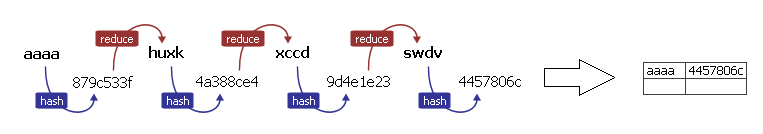
\includegraphics[scale=0.8,frame]{img/rbtprincipe.png}
             \caption{Principe d'une ligne dans une RBT}
             \label{fig:rbtprincipe}
         \end{figure}
         
         \subsubsection{Fonctions de hachage}
         La première partie d'une création de RBT est l'implémentation de fonctions de hachage\cite{WikiHachage}. L'entièreté de notre code sur les RBT étant en java, nous avons d'abord cherché si des bibliothèques de base existaient pour les fonctions de hachages les plus connues (SHA, MD5...). Et en effet, une bibliothèque comprenant ces fonctions existe, nous facilitant la tâche pour celles-ci.
         \newline
         \indent L'inconvénient de ces fonctions est qu'elles sont toutes sur un nombre de bits supérieur à 128, ce qui ne permet pas de se représenter simplement les problèmes que peuvent poser ces fonctions, tels que les collisions\footnote{Par exemple, il faudrait un mot de passe de taille > 20 pour que le nombre de mots de passe possibles sur un alphabet de taille 93 surpasse le nombre de haché possible sur 128bits ($93^{20} > 2^{128}$ > $93^{19}$)}.
         Nous avons donc choisi d'implémenter en plus une fonction de hachage sur 8 bits, le hachage de Pearson\cite{WikiPearson}.
         
         \subsubsection{Fonctions de réduction}\label{section:reductions}
         Une fois que l'on a un haché, on veut pouvoir le \textbf{réduire.} Les fonctions de réductions sont des fonctions arbitraires. Elles permettent, à partir d'une chaîne de caractère, d'obtenir une autre chaîne de caractère qui contient moins d'informations. (voir figure \ref{fig:rbtprincipe})
         \newline
         \indent Les premières fonctions de réductions auxquelles on peut penser sont tout simplement de reprendre les n première(s) lettres d'un haché, et de retourner ce haché tronqué. Il y a plein d'autres approches naïves aux fonctions de réductions, mais elle posent toutes plusieurs problèmes:
         \begin{itemize}
             \item \textbf{Les caractères autorisés: } En effet, si l'on tronque juste un haché, qui sera souvent représenté sous une forme hexadécimale, alors nos réduits ne contiendront que des caractères hexadécimaux. Or, l'utilité de ces réduits est d'avoir, à partir d'un haché, un nouveau mot de passe clair, qui peut donc contenir tous les caractères alpha-numériques.
             \item \textbf{Les variations de ces fonctions: } Il existe beaucoup de fonctions de réductions... Le problème étant de devoir les implémenter \textit{toutes.} Certaines pourraient en effet prendre un paramètre, et prendre par exemple tout les 2, 3 caractères.. mais cela resterait limité.
         \end{itemize}

         \newline
         \indent La solution au premier problème a été d'implémenter un générateur de mots qui, comme son nom l'indique, génère un mot aléatoirement. L'avantage de cette fonction de génération est que c'est du pseudo-aléatoire. Cela signifie que l'on peut mettre en paramètre une "graine" (seed en anglais) qui permettra à cette fonction de \textbf{toujours recréer le même mot pour une graine définie.}
         \newline
         \indent Pour ce qui est du second problème, une question se pose d'abord: \textit{Pourquoi est-ce un problème? Ne peut-on pas seulement avoir une fonction de réduction pour toute la table?} Cela n'est en soi pas un problème pour la création de la table en elle-même, mais ça l'est pour son efficacité. En effet, si il n'y a qu'une seule fonction de réduction, il y a deux effets possibles: 
         \begin{itemize}
             \item \textbf{Sur une ligne: } Si, à une couleur N, on retrouve après réduction le clair en couleur N-i, on rentre alors dans une boucle. La ligne cache donc beaucoup moins de nouveaux clairs que prévu.
             \item \textbf{Sur toutes les lignes: } Si on retombe sur un clair déjà trouvé sur une autre ligne, alors on aura des clairs redondants sur plusieurs lignes.(voir figure \ref{fig:rbtcollision})
         \end{itemize}

         \begin{figure}[hbt!]
             \centering
             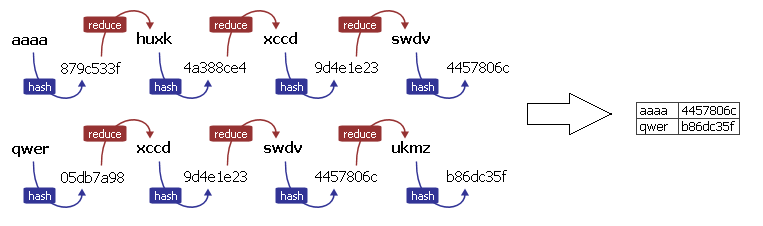
\includegraphics[scale=0.8, frame]{img/rbtcollision.png}
             \caption{Exemple de collision: la deuxième ligne tombe sur un clair déjà contenu dans la première.}
             \label{fig:rbtcollision}
         \end{figure}
         \indent Ces problèmes sont donc facilement restreints en utilisant plusieurs fonctions de réductions. Il en reste que notre approche naïve est lourde, car pour pouvoir restreindre au plus ces problèmes, il nous faut autant de fonctions de réductions qu'il y a de couleurs. En effet, si on a autant de fonctions de réductions, alors il faudrait que la redondance soit sur la même couleur pour que cela fasse un effet boule de neige sur toutes les autres couleurs. Sinon cette redondance est mitigée.
         \newline
         \indent De ce fait, pour pouvoir créer autant de fonctions de réductions que l'on veut, plutôt que d'en implémenter un nombre astronomiquement grand, on en implémente une seule, avec un nombre astronomiquement grand de paramètres différents (c'est a dire, la taille de la plage de valeur d'un int, soit $2^{32}$).
         \newline
         Voici l'implémentation en question (en java):
         \lstinputlisting[language=Java, firstline= 20, lastline= 30,frame = single, caption=Implémentation de la réduction avec graine, captionpos=b, basicstyle=\small]{code/SeededReduction.java}

         Le paramètre en question, \textit{offset}, est donc un int. Pour créer le mot, on utilise comme graine la valeur de haché, transformée en int, auquel on ajoute l'offset.

         \newline
         \indent Pour finir, lors de la création de nos RBT, on va créer autant d'objets \textbf{SeededReduction} qu'il y a de couleurs, avec pour chacun un offset incrémenté de 1 par rapport à la dernière. On a donc une fonction de réduction différente pour chaque couleur, et donc réduit les redondances le plus possible\footnote{Il serait sûrement probable de mitiger encore plus le problème en créant une fonction de réduction à chaque réduction faite, mais il y aurait donc autant de fonctions de réduction que de clairs caché dans la RBT, ce qui serait peu raisonnable..}

         \subsubsection{Génération de mots}
         Comme indiqué précédemment dans les fonctions de réduction, on a besoin d'un moyen de générer des mots aléatoires pour nos réductions... Mais aussi afin de générer des clairs de base pour nos tables. Pour ce faire nous avons implémenté un générateur basique, avec une fonction de génération prenant simplement en paramètre la taille du mot à générer, et si besoin, une graine. Cela nous permet de générer aléatoirement des bases de mots, avec une graine déterminée par le programme en lui même. De plus, il permet de générer des mots mais cette fois ci de façon déterministe, avec une graine, pour nos réductions\cite{WikiPseudoAleatoire}.
         L'importance de ce coté déterministe sera approfondie dans l'explication de l'attaque (section \ref{section:Attaque}).
         \newline
         \indent Une propriété bien utile des fonctions pseudo-aléatoires est que, comme les fonctions de hachage, lorsque la graine diffère de très peu, la génération diffère grandement. Notre offset des graines incrémentant de 1 dans les fonctions de réduction est donc suffisant.
         \subsubsection{Format des tables} \label{section:Format}
         Une fois toutes ces fonctions créées, la question qui s'est posée était le choix du format des tables. Nous avons rapidement opté pour un simple fichier texte constitué de 2 colonnes. La première pour les clairs et la seconde pour les haché. Par la suite les tables arc-en-ciels avaient l'extension \textit{.rbt} pour pouvoir bien les identifier. Ce choix d'utiliser un simple fichier texte se justifie par sa simplicité et la nécessité de devoir écrire et lire les fichiers via du code.
         \newline
         \indent Le souci de cette approche plutôt naïve pour formater les RBT est qu'un haché prend souvent une vingtaine voire trentaine de caractères sur une représentation hexadécimale. Ce qui prend largement plus de place qu'un mot de passe en clair de 10 caractères.
         Sachant que nos tests seront effectués (pour la plupart) sur des fonctions de hachages d'au moins 128bits, nous avons choisi au final de mettre dans la deuxième colonne un clair, qui correspond a la n+1ème réduction, afin de réduire la taille des RBT.
         \newline
         \indent De plus, comme nous allons le voir en section \ref{section:Attaque}, l'attaque nécessite que tous les clairs soient de la même taille pour pouvoir être effectuée (sans quoi elle serait très peu optimisée). C'est pourquoi notre représentation est finalement sous la forme d'une liste de "sous-tables", où chaque sous table est un fichier avec uniquement des clairs de taille n, définie à la création. Lors de la création, autant de fichiers sont créés que de taille différentes de clair que l'on souhaite. Cette représentation permet aussi une certaine modularité: en effet, on peut maintenant choisir le nombre de couleurs et la taille de chaque sous table.
         
         \subsection{Attaque avec une table} \label{section:Attaque}
         L'attaque avec une table se passe de cette manière:
         \begin{enumerate}
             \item On a un mot de passe haché, et une table qui a été créée avec la même fonction de hachage que le haché que l'on a.
             \item On commence avec n (notre nombre de couleurs).
             \item On effectue les réductions allant de n au nombre de couleurs sur ce haché, en re-hachant entre chaque réduction (comme lors de la création de notre table).
             \item On vérifie dans toute la 2ème colonne de notre table, si notre clair correspond à l'un d'eux.
             \item Si oui, alors on effectue les réductions 0 à n sur le clair correspondant dans la 1ère colonne, ce qui nous donne le clair qui donnerait le haché que l'on a de base. (On vérifie tout de même car il peut y avoir eu une redondance dans les réductions, surtout dans les mots de passe court)
             \item Si non, on repasse à l'étape 3, avec n-1.
             \item Si n=0 et on a toujours rien trouvé, alors l'attaque a échouée : Le haché ne se trouve pas dans notre RBT.
         \end{enumerate}
         
         \begin{algorithm}[H]
        \DontPrintSemicolon
        \SetKwData{Hache}{h}
        \SetKwData{N}{n}
        \SetKwData{Table}{RBT}
        \KwIn{Un haché $\Hache$, la table $\Table$ et la longueur de mot de passe $\N$ représentée dans la table}
        \KwOut{Le clair correspondant au $\Hache$ si trouvé, sinon rien}
        \For{$i \gets \Table.nbCouleurs$ à 0}{
            $etape \gets \Hache$ \;
            \For{$j \gets i$ à $\Table.nbCouleurs$}{
                $courant \gets \Hache$ réduit par $\Table.reduction[j]$ \;
                $etape \gets courant$ haché par la fonction de hachage de $\Table$
            }
            \uIf{$courant$ est dans la table $\Table$ à la deuxième colonne}{
                $craque \gets$effectuer les 0 a $i$ réduction sur le mot a la première colonne correspondante \;
                \uIf{$craque$ haché par la fonction de hachage de $\Table = \Hache$}{
                    \Return $craque$
                }
            }
        }
        \caption{Algorithme de recherche dans une RBT}
        \label{algo:RBTSearch}
        \end{algorithm}

        \indent On remarque bien que cet algorithme \ref{algo:RBTSearch} nécessite d'avoir des tables où la longueur représentée est la même sur chaque ligne, d'où le format établi dans la section \ref{section:Format}. Une attaque lancera donc cet algorithme sur toutes les "sous-tables". Cette représentation est donc encore avantageuse, car cela permet de ne pas avoir à retrouver la longueur à utiliser pour la réduction à chaque ligne, mais plutôt à chaque début de sous table. On évite ainsi un grand nombre d'opérations coûteuses.
        \subsection{Optimisations}
         
       \subsubsection{Les automates de Markov}
       Les automates de Markov\cite{AutomatesMarkov} permettent de générer des mots plus pertinents qu'avec une génération purement aléatoire. Ici, le but était de s'en servir pour obtenir une liste de mots de passe plus pertinents à partir desquels nous aurions construit une RBT également plus pertinente. Malheureusement, nous n'avons pu finaliser l'implémentation de cette optimisation. Nous allons cependant vous présenter son fonctionnement et notre état d'avancement sur cette partie du projet. À partir d'un corpus de mots, les automates de Markov associent une improbabilité à chaque transition entre 2 caractères, c'est-à-dire à quel point est-ce improbable d'avoir un B après un A par exemple. En utilisant ces automates et une valeur d'improbabilité maximale on peut construire un ensemble de mots qui, ici, nous servirait à construire une table. 
       \newline
       \indent Dans notre implémentation, les automates se présentent sous la forme de matrices carrées de même taille que l'alphabet utilisé plus un, pour prendre en compte le caractère vide qui correspond à l'improbabilité qu'un mot commence par la lettre. 
       \begin{figure}[hbt!]
           \centering
             $\begin{pmatrix} 
                  \textit{null}_\textit{null} & a_\textit{null} & b_\textit{null} & \cdots & z_\textit{null} \\ 
                  \textit{null}_a & a_a & b_a & \cdots & z_a \\
                  \textit{null}_b & a_b & b_b & \cdots & z_b \\
                     \vdots & \vdots & \vdots & \ddots & \vdots \\
                  \textit{null}_z & a_z & b_z & \cdots & z_z        
            \end{pmatrix}$

             \caption{Matrice d'improbabilité}
       \end{figure}  
       \newline
       \newpage
       \indent Dans cette matrice, la valeur ${a}_{null}$ correspond à l'improbabilité d'avoir un $a$ qui suit un null, c'est-à-dire l'improbabilité qu'un mot commence par un a.  
        \newline
            
          \lstinputlisting[language=Java, firstline= 94, lastline= 110,breaklines=true,frame = single, caption=Fonction Parser mettant à jour la matrice à partir d'un String]{code/TestMarkov(1).java}
       
       \indent Cet algorithme permet à partir d'un $String$ en entrée de mettre à jour le tableau $tab$ précédemment initialisé. Lors de l'initialisation, le tableau est entièrement rempli de 1, et à chaque occurrence d'un couple $current\-previous$, on rajoute 1 à la case concernée. On obtient donc une matrice comprenant le nombre d'occurrences moins 1 de chaque couple. Pour calculer les valeurs d'improbabilité, on applique à toutes les cases la formule : 
        \newline
        \begin{align}
            I = -10.log(P)
        \end{align}
          \newline
         \indent Avec \textit{P} la probabilité d'occurrence d'une lettre suivie d'une autre, c'est-à-dire la valeur de la case divisée par le nombre total de lettres utilisée pour créer le tableau. Cette formule est la raison du choix d'initialiser le tableau avec des 1 plutôt que des 0. En effet si un couple venait à ne jamais être rencontré on aurait une probabilité égale à 0 et le problème est que \textit{log}(0) n'existe pas.  
       


       \indent À partir de la matrice d'improbabilité, nous pouvons construire l'arbre des mots possibles. L'arbre est constitué de noeuds contenant chacun 2 valeurs : une lettre et un capital d'improbabilité. Ce capital d'improbabilité est un nombre arbitraire défini en amont et qui correspond à la somme des improbabilités des lettres qui constituent les mots. La racine de l'arbre est un noeud contenant le caractère $null$ et le capital d'improbabilité. Les enfants de ce noeud sont toutes les lettres qui peuvent suivre le caractère et dont l'improbabilité ne fait pas descendre le capital en dessous de 0. Ici par exemple, un enfant de cette racine sera un noeud avec le caractère $a$ et le nouveau capital vaut la valeur initiale moins la case ${a}_{null}$. On répète l'opération pour chaque enfant jusqu'à obtenir notre arbre.
        \begin{figure}[hbt!]
            \centering
             \begin{tikzpicture}
        \node {null}[sibling distance = 2cm, level distance = 1cm]
            child {node {${a}_{null}$} [sibling distance = 0.5cm, level distance = 1cm]child {node {${a}_{a}$}}
            child {node {${b}_{a}$}}
            child {node {${...}_{a}$}}
            child {node {${z}_{a}$}}}
            child {node {${b}_{null}$}[sibling distance = 0.5cm, level distance = 1cm]child {node {${a}_{b}$}}
            child {node {${b}_{b}$}}
            child {node {${...}_{b}$}}
            child {node {${z}_{b}$}}}
            child {node {${...}_{null}$}[sibling distance = 0.5cm, level distance = 1cm]child {node {${a}_{...}$}}
            child {node {${b}_{...}$}}
            child {node {${...}_{...}$}}
            child {node {${z}_{...}$}}}
            child {node {${z}_{null}$}[sibling distance = 0.5cm, level distance = 1cm]child {node {${a}_{z}$}}
            child {node {${b}_{z}$}}
            child {node {${...}_{z}$}}
            child {node {${z}_{z}$}}};
           
        \end{tikzpicture}
         \caption{Exemple d'un début d'arbre}
        \end{figure}
        \newline
   
        \indent
        
        Les mots qu'on souhaite obtenir sont l'ensemble des chemins qui mènent à une feuille. Ici par exemple, nous avons $aa$, $ab$, etc.. Cet arbre correspond à tous les mots de longueur 2 mais la profondeur de l'arbre peut être bien plus élevée et l'arbre n'est pas forcément complet.
            \newline
            \indent Dans notre implémentation, nous avons 2 algorithmes de génération d'arbres mais malheureusement par manque de temps nous n'avons pas pu correctement les tester. L'algorithme permettant d'obtenir les mots à partir des arbres est simplement un parcours en profondeur renvoyant la liste des noeuds traversés avant d'arriver sur une feuille. 
    
        
        \indent Les automates de Markov présentés précédemment permettaient d'obtenir une liste de clair pertinents mais il existe d'autre moyens d'obtenir des clairs pertinents. Par exemple, nous avons récupéré une liste du million de mots de passe\cite{CommonPassword} les plus fréquemment utilisés et cela nous permettait d'avoir une base pertinente pour créer une table. Du moins pertinente dans l'usage conventionnel des RBT, à savoir trouver des mots de passe à partir de haché. En effet avoir des mots de passe couramment utilisés augmente la chance de succès. 

        \subsubsection{VisualVM\cite{VisualVM}}\label{section:VisualVM}
        VisualVM est un outil de profiling sur la machine virtuelle java\cite{VMJava}, ce qui permet de récolter des données sur l'exécution du code sur cette machine virtuelle, y compris le temps passé sur certaine fonctions. Cela nous a permis de nous rendre compte de quelques pratiques plutôt coûteuses en temps, comme l'utilisation de la fonction \textit{split(String regex)} d'un String, que l'on utilisait dans la fonction $isInTable()$ de $RainbowTableCracker$ (cf: figure \ref{fig:diartables}), afin de séparer chaque ligne en deux colonnes.
        Nous l'avons donc remplacée par la fonction \textit{substring(int beginIndex, int endIndex)}, que l'on pouvait utiliser car les clairs font tous la même taille dans notre sous-table, ce qui veut dire que la second colonne commence toujours à l'index $taille+1$ et finit à l'index $(taille*2)+1$
         
         
         Une seconde fonction prenait cependant encore plus de temps lors des expérimentations à la base: le \textit{readline()} de notre $BufferedReader$\cite{BuffReader}\footnote{En réalité, la création de ces $BufferedReader$ était aussi très coûteuse, car répétée un grand nombre de fois, mais ce problème est résolu en réglant le problème du \textit{readline()}}
        En effet, le problème était que pour chaque mot de passe (haché) testé lors des expérimentations, la table était relue ! Or, c'est très inefficace, surtout lorsque l'on trouve un nombre très restreint de mots de passe, ce qui implique que la recherche ne s'interrompt pas en plein milieu de la table.

        
        C'est pour cela que l'on a implémenté les fonctions $isInTableBulk()$ et $crackHashBulk()$ (ainsi que les autres fonctions sous-jacentes, voir figure \ref{fig:diartables}), qui permettent de rechercher \textbf{tous} les mots de passes souhaités d'une seule lecture de table. Cela implique une expérimentation plus gourmande en mémoire, mais qui est en théorie accélérée par un facteur \textit{nombre de mot de passe recherché}. Ce coût en mémoire fera malheureusement du tort à une certaine expérimentation, voir section \ref{section: exp}.
        De plus, notre implémentation doit tout de même relire la table pour chaque couleur de celle-ci, ce qui serait, théoriquement résoluble, mais aurait un coût en mémoire encore plus élevé. Il serait tout de même possible d'implémenter cette optimisation (1 seule lecture de table pour toutes les couleurs) dans les fonction recherchant 1 seul haché à la fois. 
        
        
        
        \subsubsection{Expérimentations en multi-thread}
        Lors des expérimentations, nous nous sommes rendus compte que l'algorithme ne tournait que sur un seul coeur du processeur de la machine, ce qui allonge considérablement le temps de calcul. Or, chaque expérimentation n'ayant aucune influence sur une autre, elle sont donc chacune par définition parallélisable. Toutes les exécuter en même temps sur le même coeur ne servirait évidemment a rien, c'est pour cela que l'on va exécuter une expérimentation par coeur de la machine. Pour cela, on va utiliser l'interface $Runnable$\cite{Runnable} ainsi que l'objet $ExecutorService$\cite{ExeService}. Le premier sert à rendre notre fonction exécutant l'expérimentation "Runnable", c'est à dire qu'elle pourra être exécutée et gérée par le second, notre $ExecutorService$. Notre fonction d'expérimentation est donc maintenant un processus, dont on peut attendre la fin de son exécution -ou pas- avant d'en lancer une autre. En fixant le nombre de processus autorisé à être exécuté par $ExecutorService$ avec le nombre de coeurs $n$ disponible sur notre machine\footnote{Plus précisément sur l'environnement courant de notre machine virtuelle java\cite{VMJava}}, cela nous permet d'exécuter $n$ expérimentations en même temps nous offrant en théorie un speedup de $n$. En pratique, nous avons besoin de barrière(s) de synchronisation dans nos expérimentations, plus précisément à la fin de chaque type d'expérimentation, afin principalement de pouvoir fermer les flux d'écritures sur nos fichiers de résultats d'expérimentations, ce qui réduit inévitablement ce speedup théorique, mais cela reste négligeable.

    \section{Architecture du projet}
    \subsection{Diagrammes de classe}


    \begin{figure}[H]
             \centering
             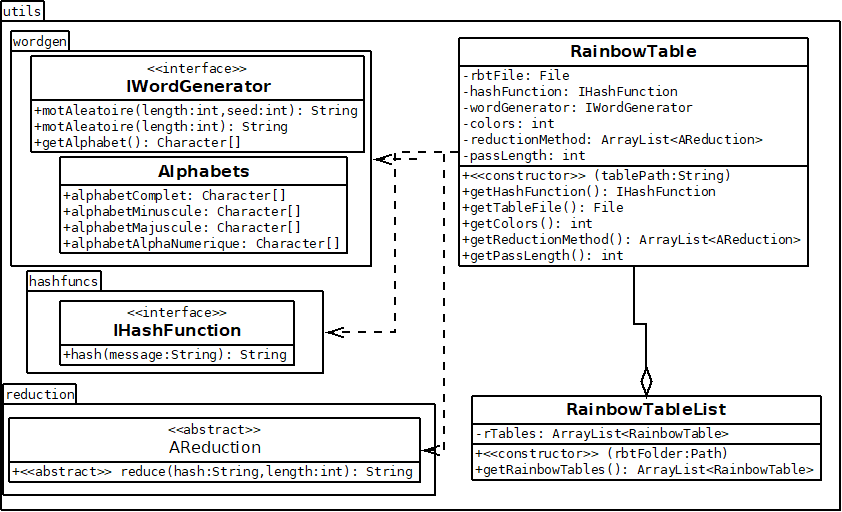
\includegraphics[scale=0.5, frame]{img/diagrams/utils.png}
             \caption{Diagramme de classe du package $utils$}
             \label{fig:diautils}
    \end{figure}

    Le package $utils$ (figure \ref{fig:diautils}) contient toutes les fonctions utilitaires de notre projet, y compris la représentation sous forme d'objet d'une RBT (la classe $RainbowTableList$). Cette représentation contient une liste de $RainbowTable$, qui sont la représentation des "sous-tables". Ces sous tables sont construites uniquement à partir de leur fichier, avec lequel on récupère les paramètres de celle-ci, et on les attribue dans son constructeur.
    
    \begin{figure}[H]
             \centering
             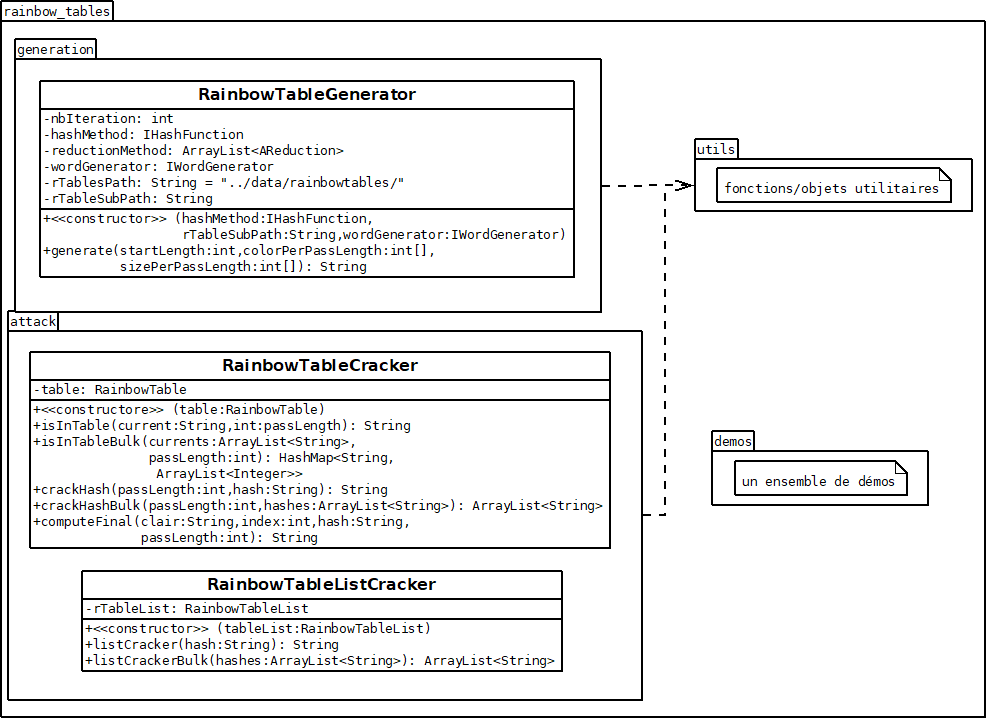
\includegraphics[scale=0.5, frame]{img/diagrams/rainbow_tables.png}
             \caption{Diagramme de classe du package $rainbow\_tables$}
             \label{fig:diartables}
    \end{figure}

    Le package $rainbow\_tables$ (figure \ref{fig:diartables}) contient les paquets $generation$, $attack$, $utils$ et $demo$:
    \begin{itemize}
        \item \textbf{generation}: contient les fonctions relatives à la génération d'une RBT.
        \item \textbf{attack}: contient les fonctions relatives à l'attaque d'une RBT. Séparée en deux objets, l'un représentant l'attaque sur une "sous-table", l'autre sur une RBT entière. (Le second utilise le premier).
        \item \textbf{demos}: contient des démos variées.
    \end{itemize}
    
    \subsection{Chaînes de traitement}
    Les fonctions de génération de RBT utilisent les fonctions de réduction, hachage et de génération de mots, car nécessaires pour créer des RBT (voir section \ref{section:creationRBT}). Les fichiers créés sont utilisés dans les fonctions d'attaques, où elles sont représentées sous un objet $RainbowTableList$ (figure \ref{fig:diautils}). L'attaque utilise de plus les fonctions de réduction, car nécessaire pour celle-ci (voir section \ref{section:Attaque}).
    \newline \indent Les fonctions de réduction quant à elle, utilisent aussi les fonctions de génération de mots, comme vu en section \ref{section:reductions}.
    

        \newpage
    \section{Expérimentations} \label{section: exp}
    Le but des expérimentations était de trouver quel paramètre influe sur l'efficacité des RBT. Les trois paramètres que nous pouvons faire varier sont la taille de la table (le nombre de mots de passe inscrits à l'intérieur de la table), le nombre de couleurs (le nombre de réductions par mot de passe) et enfin la taille des mots de passe. Dans un but que les expérimentations soient le plus exhaustive possible, ces trois paramètres sont chacun testés avec des variations sur les deux paramètres restants. Les graphes présentés dans les sections suivantes sont par trois, car nous avons testé 3 fonctions de hachage différentes: MD5\cite{WikiMD5}(avec une taille d'empreinte de 128bits, SHA3\cite{WikiSHA3} (avec une taille d'empreinte de 512bits) et Pearson\cite{WikiPearson}(avec une taille d'empreinte de 8 bits)\footnote{Nous avions implémenté d'autre fonctions de hachage, mais les résultats entre MD5 et SHA3 étant déjà similaire, nous ne trouvions pas l'utilité de les tester aussi.}.

    Les paramètres utilisés pour les tests sont les suivants:
    
    \begin{tabular}{|c|c|c|c|}
        \hline
         & Taille MDP & Nombre de couleurs & Taille de la table  \\
         \hline
         Var Taille MDP & x & {3, 4, 5, 6} & {3, 4, 5, 6} \\
         \hline
         Var nb couleurs & {1, 2, 4, 7, 10, 20} & x & {1, 2, 4, 7, 10, 20} \\
         \hline
         Var taille table & {1000, 2000, 5000, 10000} & {1000, 2000, 5000, 10000} & x\\
         \hline
    \end{tabular}

    La taille de mot de passe commence à trois pour se rendre compte d'un cas d'école qui est qu'un mot de passe de taille trois n'est vraiment pas sécurisé.

    Les valeurs "constantes", c'est à dire, les valeurs utilisées pour le paramètre restant dans une expérimentation :
    \begin{itemize}
        \item \textbf{Taille des mdp:} 4. Cela permet d'avoir une plage de mots de passe de $26^4$, suffisante pour les tests. Une taille de 3 aurait été trop petite et les résultats n'auraient que très peu de sens.
        \item \textbf{Nombre de couleurs:} 3. Cela permet d'avoir un test plus concluant sans rallonger trop le temps de calcul, puisque de toute façon ce n'est pas le paramètre testé.
        \item \textbf{Taille de la tables:} 10000. De même que pour les couleurs, cela permet un test plus concluant sans rallonger le temps de calcul plus qu'il ne le faut.
    \end{itemize}

    Le nombre de mots de passe testés sur chaque variation dépend de si la taille des mots de passe est un paramètre fixé ou non. Cela reste un pourcentage, mais, si la taille des mots de passe varie, on teste un nombre de 0.01\% de la taille de la plage de mots de passe de la taille courante. Cela permet d'avoir à tester environ $300000$ mots de passe lorsque la longueur est au plus haut, c'est à dire 6 (c'est aussi pour cela que l'on ne teste pas de plus grande longueur de mot de passe). En revanche, si la taille des mots de passe est fixé, alors on test 30\% de la taille de la plage. En effet, notre paramètre fixe étant $4$, cela nous donne environ $130000$ mots de passe à tester.
    
    \subsection{Tests sur la taille des tables}
    
     Ces graphes (figure \ref{fig:TSC} et \ref{fig:TCS}) présentent les résultats des expérimentations où le principal paramètre variant est la taille des tables. Pour le premier couple de graphe, on constate que l'augmentation de la taille de la table augmente le taux de réussite de l'attaque mais principalement pour les petits mots de passe. A partir d'une longueur de mot de 5, la table arrive à peine à obtenir des résultats. Donc augmenter la taille de la table n'est pas suffisant pour efficacement craquer des mots de passe long. Le second couple de graphe nous montre une variation de la taille de la table couplé à une variation du nombre de couleur. Ici l'augmentation du taux de réussite est assez évidente puisque la taille du mot de passe est assez petite et on fait augmenter les 2 autres paramètres. On peut cependant remarquer que l'augmentation (passé 10 000) est très similaire pour toutes les courbes. Ce qui montre une certaine limite des gains obtenables grâce à l'augmentation de la taille de la table. Il faut également noter qu'augmenter la taille de la table la rend plus lourde. Dans le compromis temps-espace lié à la question de l'efficacité des RBT, cette solution sacrifie de l'espace.
    
     \begin{figure}[H]
     \centering
    
      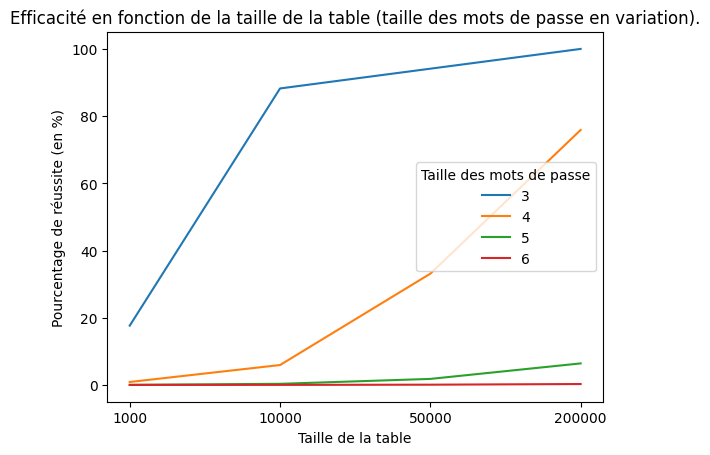
\includegraphics[scale=0.9]{img/graphe/md5/T_S_C_100000_MotGenerator.png}
    
    
      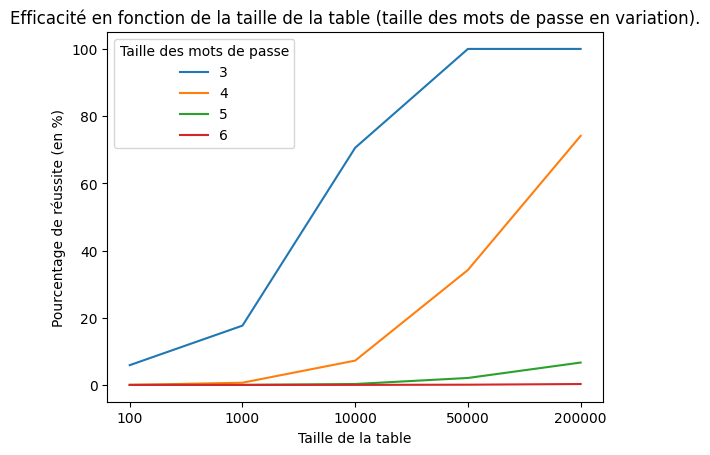
\includegraphics[scale=0.9]{img/graphe/sha3/T_S_C_100000_MotGenerator.png}
    
   
    \caption{Expérimentations sur MD5 et SHA3 (de haut en bas)}
    \label{fig:TSC}
    \end{figure}
    
    \begin{figure}[H]
                
    
      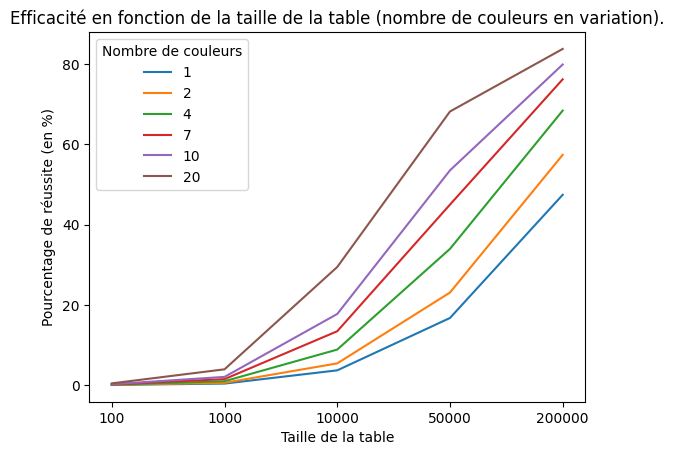
\includegraphics[scale=0.9]{img/graphe/md5/T_C_S_137092_MotGenerator.png}
   
    
      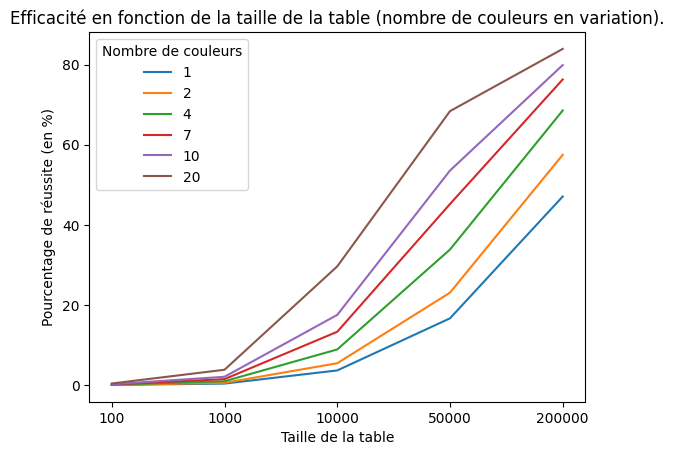
\includegraphics[scale=0.9]{img/graphe/sha3/T_C_S_137092_MotGenerator.png}
   
    \hspace{0mm}
    
    \caption{Expérimentations sur MD5 et SHA3 (de haut en bas)}
    \label{fig:TCS}
    \end{figure}

    On remarque que les résultats sur le hachage de Pearson ne sont pas présents. En effet, lors des expérimentations, les tests sur la taille de la table n'arrivaient tout simplement pas à aboutir, dû à notre implémentation. Mais on va vite remarquer avec les expérimentations suivantes que Pearson est vraiment peu sécurisé, avec ces empreintes à 8bits.

    \newpage
    \subsection{Tests sur le nombre de couleur}
   
         \begin{figure}[hbt!]
                \centering
   
      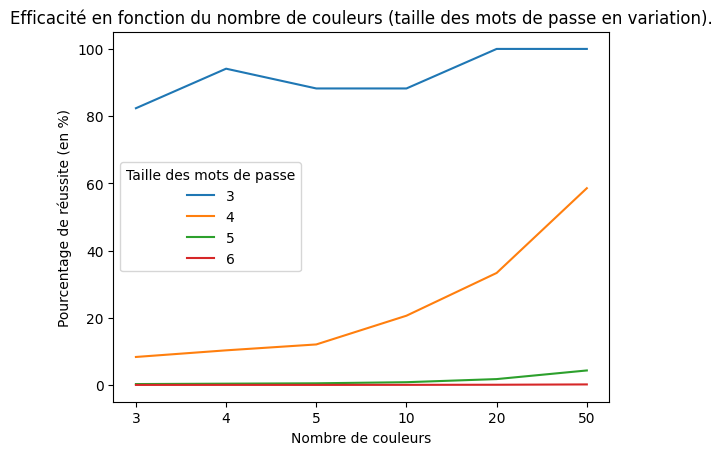
\includegraphics[scale=0.65]{img/graphe/md5/C_S_T_100000_MotGenerator.png}
  
    
      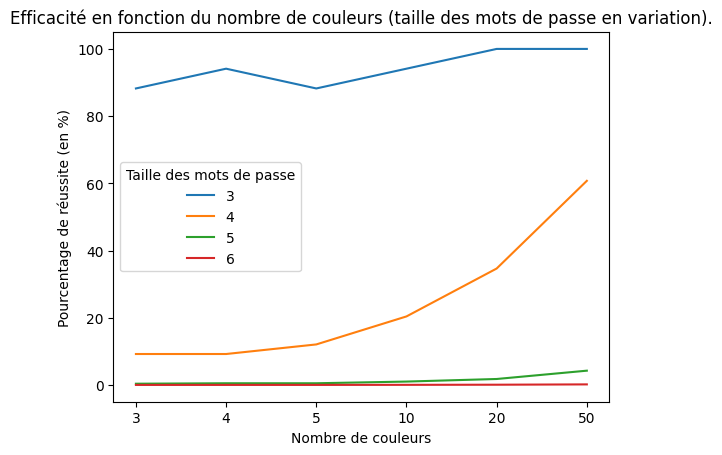
\includegraphics[scale=0.65]{img/graphe/sha3/C_S_T_100000_MotGenerator.png}

      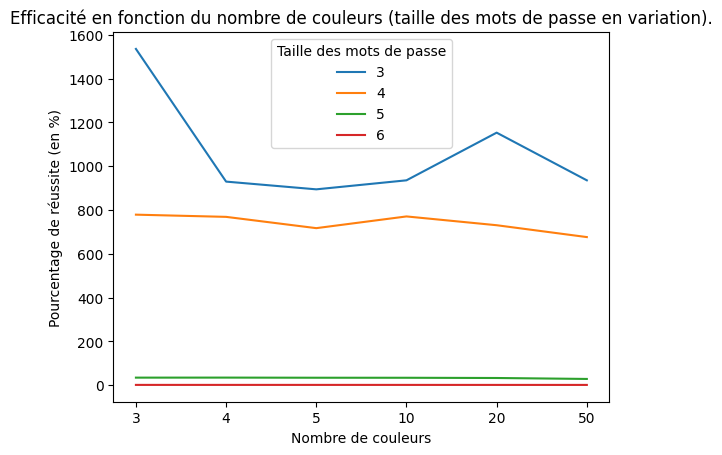
\includegraphics[scale=0.65]{img/graphe/pearson/C_S_T_100000_MotGenerator.png}
    
    \hspace{0mm}
    
    \caption{Expérimentations sur MD5, SH3 et Pearson (de haut en bas)}
    \label{fig:CST} 
    \end{figure}
    
    \newpage
     \begin{figure}[hbt!]
     \centering
    
      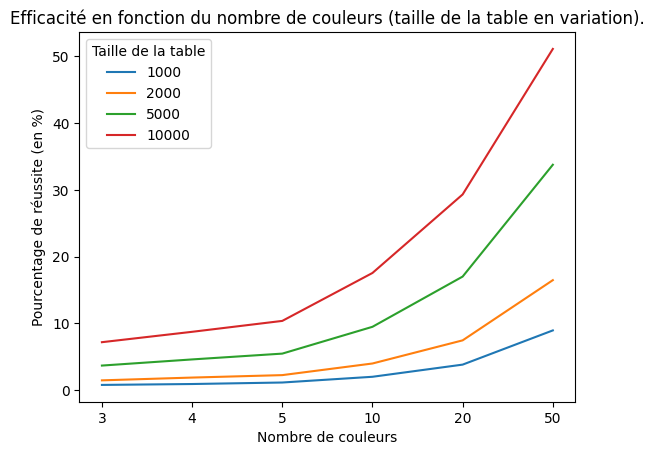
\includegraphics[scale=0.65]{img/graphe/md5/C_T_S_137092_MotGenerator.png}
    
      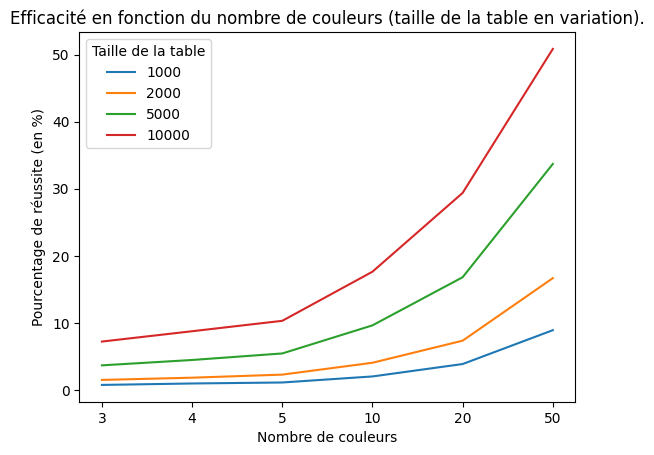
\includegraphics[scale=0.65]{img/graphe/sha3/C_T_S_137092_MotGenerator.png}

      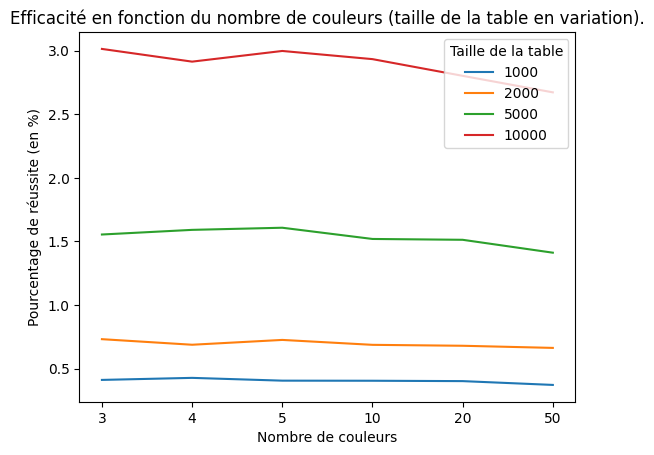
\includegraphics[scale=0.65]{img/graphe/pearson/C_T_S_137092_MotGenerator.png}

    \caption{Expérimentations sur MD5, SH3 et Pearson (de haut en bas)}
    \label{fig:CTS}
    \end{figure}
    
    \newpage
    
    Cette fois-ci, on s'intéresse à la variation du nombre de couleurs dans la table, c'est a dire le nombre de réductions pour chaque mot de passe. Le premier couple de graphe (figure \ref{fig:CST}) nous montre une variation sur les couleurs et la taille des mots de passe avec une taille de table fixée à 10 000. Pareillement à la variation sur la taille, on constate que l'attaque est très peu efficace pour les mots de passe plus longs. On peut cependant noter la présence d'un plateau à 100\%àa partir de 20 couleurs pour les mots de passe de longueur 3 ainsi qu'une pente très élevée pour ceux de longueur 4. Cette augmentation est dû au fait que lorsqu'on ajoute une couleur cela revient à doubler le nombre de mots de passe présents dans la RBT. 
    
    
    Le deuxième couple (figure \ref{fig:CTS}) est très similaire au deuxième couple des premiers tests (figure \ref{fig:TCS}), mais ici l'augmentation est différente entre les courbes et plus le nombre de couleurs est grand plus la pente est grande, ce qui montre qu'augmenter les couleurs est assez pertinent pour obtenir des résultats.
    Cependant l'algorithme d'attaque procède couleur par couleur, donc plus le nombre de couleurs est élevé plus le temps de calcul est grand. Ce que l'on gagne en espace avec une table plus petite, on le perd en temps de calcul. C'est l'autre versant du compromis temps-espace propre aux RBT.

    On remarque que dans les deux cas, les tests sur Pearson donne des résultats très peu pertinents: un pourcentage allant jusqu'à 1600\%, et l'autre jusqu'à seulement 3\%. Cela vient du fait que ce pourcentage est calculé avec le nombre de \textbf{mots de passe trouvés}, pas d'empreintes trouvées. Or, la fonction de Pearson n'ayant que 256 empreintes en tout, on se doute que la table est suffisamment grande pour contenir toutes les empreintes de Pearson. Par conséquent, dès qu'il y a une collision, l'algorithme tente d'ajouter le mot de passe trouvé, pas le haché. De toute façon, à partir du moment où plus de 256 mots de passes sont trouvés, cela veut dire que toutes les empreintes sont trouvées.
    
     \subsection{Tests sur la taille des mots de passe}

    Comme nous avons pu constater précédemment, l'algorithme d'attaque perd beaucoup en efficacité avec les mots de passe plus longs. Sur ces 6 graphes on constate bien qu'à partir d'une taille de 5, les résultats obtenus sont insignifiants et même presque complètement absents pour 6. L'alphabet que nous avons utilisé pour les expérimentations est uniquement constitué des lettres minuscules donc 26 caractères, par conséquent pour les mots de longueur n il y a $26^n$ mots possibles. Donc plus les mots sont longs, moins il y a de chances que le mot recherché soit dans la table sauf si l'on augmente la taille de celle-ci. C'est ce que l'on constate sur les graphes, les courbes présentant les chances de réussite les plus élevées sont celles où la table est la plus grande, que cela soit par une augmentation de sa taille ou de son nombre de couleurs. Au début de nos expérimentations, nous utilisions un alphabet beaucoup plus complet comprenant les lettres minuscules, majuscules, les chiffres et les caractères spéciaux présents sur le clavier, soit une taille de 93, mais nous nous sommes rendus compte que les résultats obtenu n'étaient pas probants et les taux de réussite étaient très faibles. Nous avons ensuite progressivement réduit la taille de l'alphabet jusqu'à obtenir des résultats plus satisfaisants. Cependant même avec un alphabet assez réduit on se rend compte que la taille des mots à un très grand impact sur l'efficacité des tables.



   \begin{tabular}{|c|c|c|c|c|c|}
        \hline
         & 3 & 4 & 5 & 6 \\
         \hline
         Minuscules & 17 576 & 456 976 & 11 881 376 & 308 915 776 \\
         \hline
         Minuscule/Majuscule & 140 608 & 7 311 616 & 380 204 032 & 19 770 609 664 \\
         \hline
         Alphanumérique & 238 328 & 14 776 336 & 916 132 832 & 56 800 235 584\\
         \hline
         Complet & 804 357 & 74 805 201 & 6 956 883 693 & 646 990 183 449 \\
         \hline
         
    \end{tabular}

    Ce tableau est à titre indicatif et il contient le nombre de mots possibles en fonction du type d'alphabet et de la longueur des mots. 

    
     \begin{figure}[H]
                \centering
  
      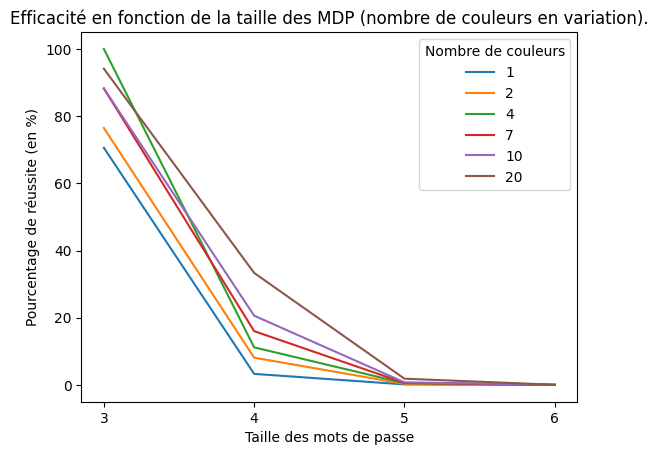
\includegraphics[scale=0.7]{img/graphe/md5/S_C_T_100000_MotGenerator.png}
  
    
      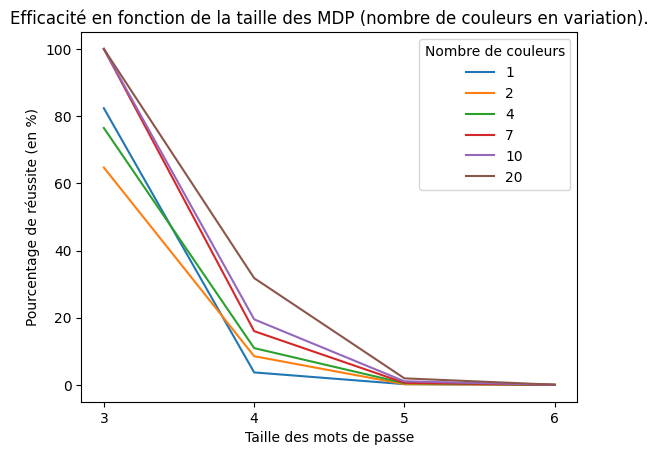
\includegraphics[scale=0.7]{img/graphe/sha3/S_C_T_100000_MotGenerator.png}

      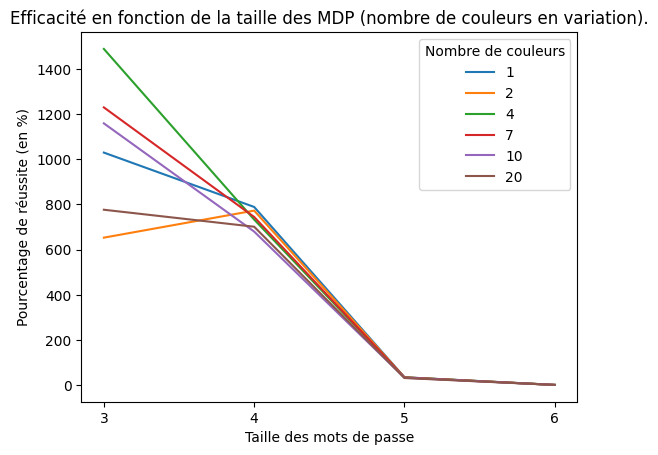
\includegraphics[scale=0.7]{img/graphe/pearson/S_C_T_100000_MotGenerator.png}
  
    \hspace{0mm}
    
    
    \caption{Expérimentations sur MD5, SH3 et Pearson (de haut en bas)}
    \end{figure}
    



    \begin{figure}[H]
    \centering
 
      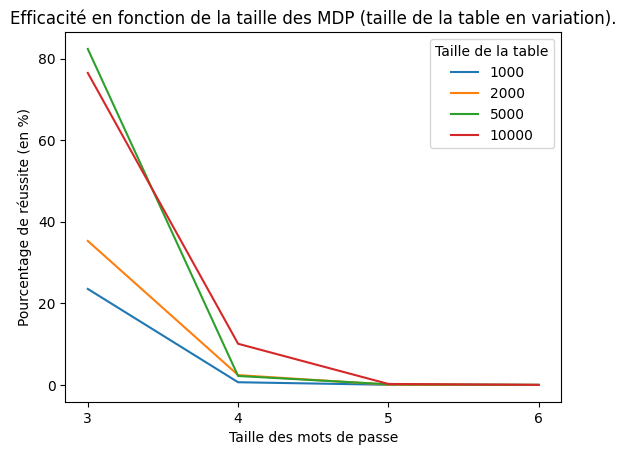
\includegraphics[scale=0.7]{img/graphe/md5/S_T_C_100000_MotGenerator.png}

    
      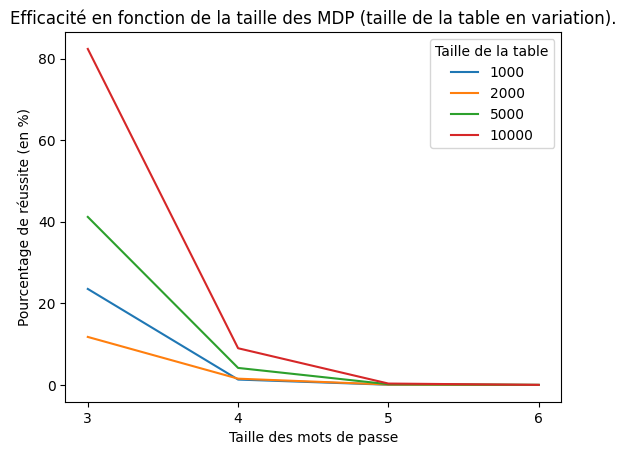
\includegraphics[scale=0.7]{img/graphe/sha3/S_T_C_100000_MotGenerator.png}

      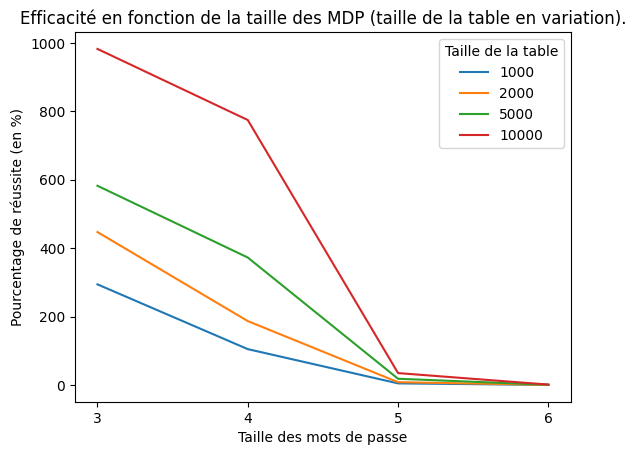
\includegraphics[scale=0.7]{img/graphe/pearson/S_T_C_100000_MotGenerator.png}

    \hspace{0mm}
    
    
    \caption{Expérimentations sur MD5, SH3 et Pearson (de haut en bas)}
    \end{figure}

    On s'aperçoit encore que pour Pearson, les résultats sont peu pertinents, pour la même raison qui a été évoquée précédemment.

   \subsection{Conclusion et analyse sur les expérimentations}
À travers nos expérimentations, nous avons pu constater les différents paramètres impactant les RBT. Ils sont au nombre de quatre: la taille de la table, le nombre de couleurs, la taille des mots de passe et la taille de l'alphabet utilisé. Pour ce qui est de la taille de la table, nous avons remarqué que l'augmenter permet une hausse de l'efficacité mais également une taille de fichier plus importante donc un coût en espace plus important. Ensuite, pour le nombre de couleurs, il permet également d'améliorer l'efficacité des tables mais cette fois cela augmente le temps de calcul nécessaire à la complétion de l'attaque. Les 2 derniers facteurs influant sur les RBT fonctionnent conjointement puisque ensemble ils définissent le nombre total de mots qui peuvent être présents dans la table : $\textit{tailleAlphabet}^\textit{tailleMot}$. Plus une table sera grande, plus elle couvrira de mots, par conséquent si on l'agrandit sans changer le nombre de mots le taux de réussite augmentera et conjointement si la table reste la même et que l'on réduit le nombre de mots alors le taux augmentera également. Construire une RBT efficace est donc un jeu d'équilibriste dans lequel il faut jouer avec les différents paramètres en fonction des besoins.
        

    \section{Conclusion}

\subsection{Récapitulatif de la problématique et réalisations}
Le projet consistait à résoudre une question scientifique : \textbf{Quelle est l'efficacité de la table en fonction du nombre de couleurs, de sa taille et de la taille des mots de passe ?}. 

Pour commencer à répondre à cette question, nous devions implémenter les objets dont nous avions besoin. Nous avons pour cela construit des RBT ainsi que tous les éléments qu'elles nécessitent (fonctions de hachage, fonctions de réduction, génération de mots, base de mots de passe clair). Avec tous ces éléments, nous avons été en mesure de générer des RBT. 

Ensuite, il nous fallait pouvoir craquer des mots de passe dans nos tables. Nous avons donc implémenter un algorithme qui cherche une empreinte dans nos tables. Nous avons par la suite mis en place un script qui créé les tables avec des paramètres (passé en argument) et qui cherche un mot de passe dans ces tables. Ce script nous a servi pour réaliser les expérimentations. 

De plus, nous avons mis en place un principe de multi-threading. Il nous a permis de faire nos expérimentations en utilisant plusieurs processus au lieu d'un seul, ce qui a grandement augmenté l'efficacité. 

Enfin, nous avons commencé à implémenter les automates de Markov pour nous permettre de créer des tables avec des mots plus pertinents.

\subsection{Résultats}

Nous avons effectué des expérimentations sur les RBT en faisant varier trois paramètres: la taille de la table, la taille des mots de passe et le nombre de couleurs. 

De ces résultats, nous avons constaté que l'augmentation d'un de ces paramètres augmente l'efficacité de la RBT. Néanmoins, l'augmentation des paramètres influe sur le poids du fichier qui contient la table ainsi que sur le temps de calcul. 

Donc, pour avoir une RBT efficace, il faut parvenir à trouver le juste équilibre entre ces deux paramètres.


\subsection{Améliorations possibles}

Nous pourrions améliorer notre programme en finalisant l'ajout des filtres Markoviens. Cette optimisation nous aurait permis d'avoir des RBT avec des mots plus pertinents. Cela augmenterait de plus l'efficacité de celle-ci.

Nous aurions pu de plus implémenter l'optimisation sur l'attaque évoquée en section \ref{section:VisualVM}, mais elle n'était pas nécessaire pour nos expérimentations.


\bibliographystyle{unsrt}
\bibliography{resources/references.bib}

\end{document}


